% !TEX root = BusSim.tex
\section{Numerical experiment}
\label{s:experiments}
\subsection{Experiment set up}

To generate the synthetic `historical' and `real-time' GPS data used in BusSim-deterministic and BusSim-stochastic, we predetermine a set of model parameters to generate realistic GPS data. Table \ref{tab:param} lists the fixed parameters being used in this experiment. 

\begin{table}[htbp]
  \centering
  \caption{Fixed parameters in BusSim-truth}
    \begin{tabular}{rll}
    %\toprule
    \multicolumn{1}{l}{\textbf{Class}} & \textbf{Parameter} & \textbf{Value} \\
    \midrule
    \multicolumn{1}{l}{Bus} & FleetSize  & Unique ID of the bus agent \\
          & Acceleration & 3 $m/s^2$ \\
          & [$\theta_1,\theta_2,\theta_3$] & [3,1,0.85] $s$ \\
    \midrule
    \multicolumn{1}{l}{BusStop} & Number of Stops & 20 \\
          & Length between stops & 2000m \\
          & GeoFence & 50m \\
    \bottomrule
    \end{tabular}%
  \label{tab:param}%
\end{table}%

Second, the dynamic parameter set $S_t = [Arr_m^t \ Dep_m^t \ V^t]$ (Equation \ref{eq:S}) are time-varying and therefore, randomly generated using fixed rules. We first generate an initial arrival rate $Arr_m^0$ at stop $m$ at time 0 by a random generation from an uniform distribution between the minimum and maximum passenger arrival rate [$minDemand, maxDemand$]. 
  
  \begin{equation}
   Arr_m = \mathcal{U} (minDemand, maxDemand) \quad m = 1,...,M
   \label{eq:arrival_rate}
\end{equation}

The departure rate is also generated from an uniform distribution, but also ordered non-decreasingly to represent the fact that more passengers alight at the end of the route than at the beginning. The departure rate at the last stop (stop M) is set as 1 to let every remaining passengers to alight the bus at the last stop. 
\begin{equation}
   Dep_m =  ordered \ (\mathcal{U} (0.05, 0.5)), \quad Dep_M = 1 \quad \& \quad m = 1,...,M
     \label{eq:departure_rate}
\end{equation}

\subsection{The stochastic and dynamic nature of BusSim-truth}

Figures  \ref{fig:2stochastic} and \ref{fig:2dynamic} provide a simple verification that demonstrates BusSim-truth generates realistic synthetic GPS data under different sets of parameters. Other variables have also been verified and will be used in the sensitivity analysis. This section outlines how this validation was achieved.

\begin{figure}[h]
	\centering
	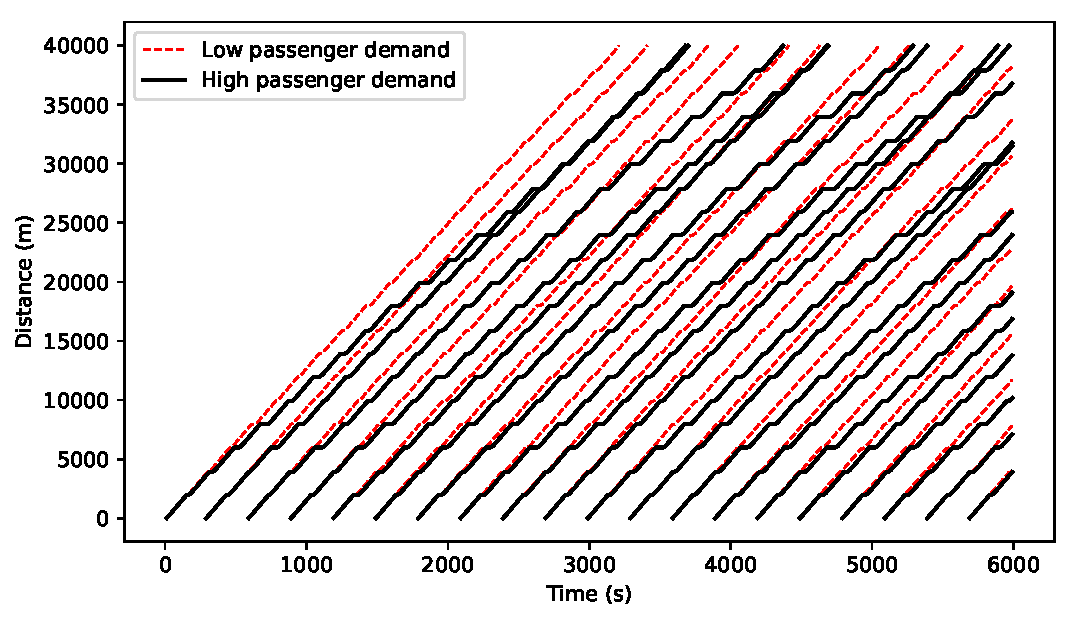
\includegraphics[width=1\textwidth]{Figures/Fig_spacetime_2stochastic.pdf}
	\caption{Synthetic bus GPS trajectory at low and high passenger demand. Red, dashed lines are bus trajectories when $maxDemand$ equals 0.5, while black, solid lines are bus trajectories when $maxDemand$ equals 2.}
	\label{fig:2stochastic}
\end{figure}

\begin{figure}[h!]
	\centering
	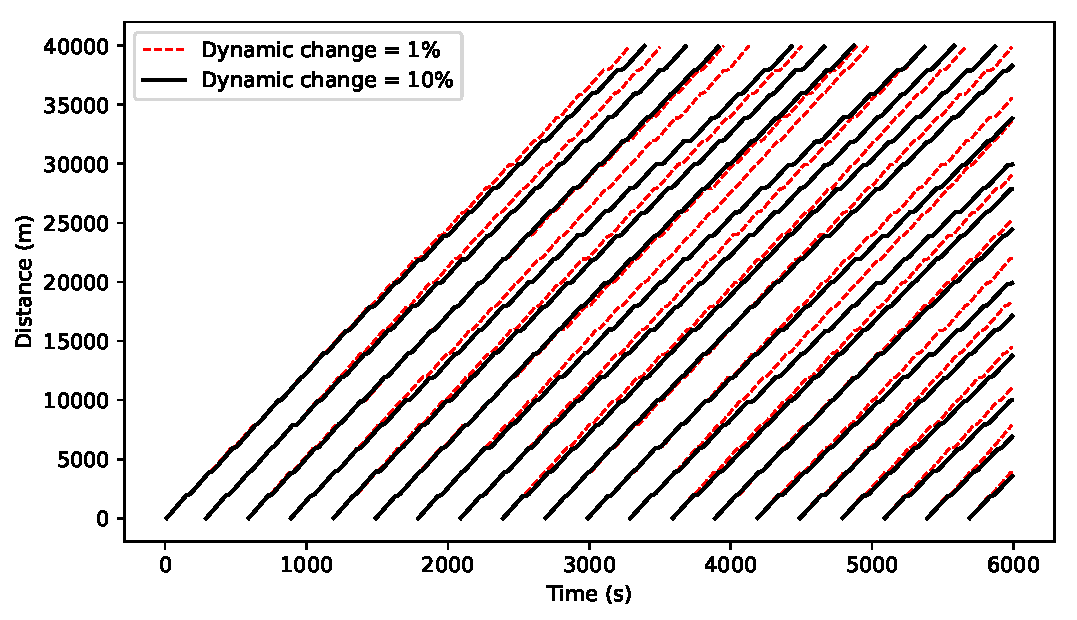
\includegraphics[width=1\textwidth]{Figures/Fig_spacetime_2dynamic.pdf}
	\caption{Synthetic bus GPS trajectory with two different value of $\xi$.}
	\label{fig:2dynamic}
\end{figure}

We aim to control the stochastic and dynamic level in BusSim-truth using only a single parameter for each. Equation \ref{eq:arrival_rate} controls the level of stochasticity in BusSim-truth. For instance, a pair of values [$minDemand, maxDemand$]=[0.5,1] means 0.5 to 1 passenger arriving at the bus stop each minute. By fixing the $minDemand$ to be a small number (e.g. equals 0.5), we can control the stochasticity of BusSim-truth by a single parameter $maxDemand$, with a larger $maxDemand$ meaning more stochasticity and vice versa. We control the level of dynamicity in BusSim-truth by a dynamic change rate parameter $\xi$, which gradually changes the arrival rate and surrounding traffic speed over the simulation period. 

To implement an inner verification of the BusSim-Truth model and to investigate the impacts of the \textit{stochastic} and \textit{dynamic} natures of the system under study, we evaluate the outputs from BusSim-truth under different values of stochasticity and dynamicity. Figure \ref{fig:2stochastic} gives an insight into the differences in bus trajectories when $maxDemand$ equals 0.5 and 2. Note that when $maxDemand$ equals 0.5, BusSim-truth reduces to a deterministic model (similar to BusSim-deterministic) because $maxDemand$ would then be equal to $minDemand$. 

Each line in Figure \ref{fig:2stochastic} shows the GPS trajectory of bus location, as generated by BusSim-truth. The solid lines show the trajectory of buses at high and stochastic demand ($maxDemand$ equals 3), whereas the dashed lines are for low and deterministic demand ($maxDemand$ equals $minDemand$). The trajectories in Figure \ref{fig:2stochastic} show that as the $maxDemand$ increases, there are more delays for each individual buses and less likely that buses are able to keep stable headway from each other. 

The dynamic nature of BusSim-truth is illustrated in 
Figure \ref{fig:2dynamic} when the dynamic change rate parameter $\xi$ is equal to 1\% and 10\%. Because the arrival rate and traffic speed gradually change, there is little change in the bus trajectories of BusSim-truth with $\xi$ equals 1\% and 10\%. As time passes, there are more delays for BusSim-truth with $\xi$ equals 10\%. This is because there are more passengers (higher arrival rate) and the buses are also travelling slower (lower traffic speed).

\subsection{Scenario 1: no calibration (benchmark)} 

This scenario aims to evaluate the prediction results from BusSim-deterministic and BusSim-stochastic \textit{without} calibrating their parameters or performing data assimilation. This is necessary so that later we can evidence the additional predictive performance of the model after calibration \textit{and} data assimilation. The two models are implemented using random parameters generated from Equation \ref{eq:arrival_rate} and \ref{eq:departure_rate}. The outputs from these models are bus locations at each time step $t$, which can be compiled to space-time trajectories and compared to the synthetic `real-time' bus trajectories, as illustrated in Figure \ref{fig:do_nothing}. 

\begin{figure}[h]
    \centering
    
\includegraphics[width=1\textwidth]{Figures/Fig_do_nothing_IncreaseRate_7.pdf}
    \caption{Prediction results from Scenario 1: no calibration}
    \label{fig:do_nothing}
\end{figure}

Figure \ref{fig:do_nothing} shows one particular case where $maxDemand$ equals 2, and $\xi$ equals 7\%, as an example of the prediction results. Both models poorly predict the trajectories of the `real' buses. This is expected because the models do not have the optimal parameters to capture the bus route operations. These models are therefore not useful for real-time prediction without parameter calibration or data assimilation. 

\subsection{Scenario 2: Parameter calibration}

In this scenario, BusSim-deterministic and BusSim-stochastic are calibrated using the Cross-Entropy Method, as described in Section \ref{s:calibration}. The two calibrated models are used to predict the bus locations at each time step $t$, which can be compiled to trajectories. Figure \ref{fig:calibration} shows an example of the comparison between the predictions from BusSim-deterministic and BusSim-stochastic versus the synthetic `real-time' GPS data, where the $maxDemand$ equals 2 and $\xi$ equals 7\%. 

\begin{figure}[htb]
    \centering
    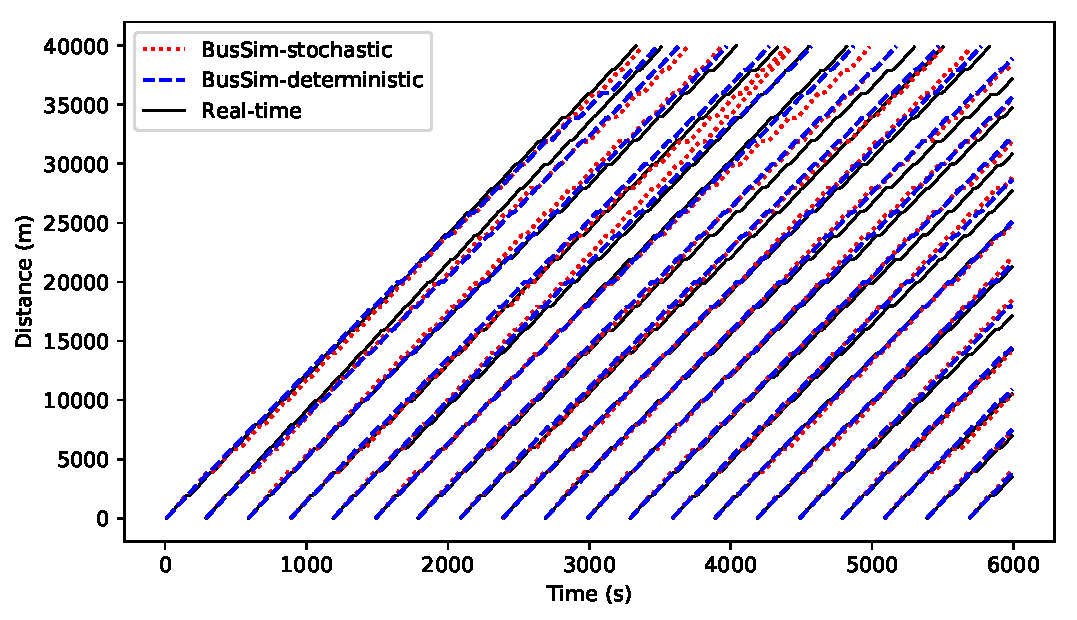
\includegraphics[width=1\textwidth]{Figures/Fig_calibration_IncreaseRate_7.pdf}
    \caption{Prediction results from Scenario 2: Parameter calibration}
    \label{fig:calibration}
\end{figure}

Although they are improvements compared the un-calibrated versions -- Figure \ref{fig:calibration} shows that both models outperform the models in the Scenario 1 (no calibration [see Figure \ref{fig:do_nothing}]) -- the models can only predict well early in the simulation when there is little deviation in passenger arrival rate and surrounding traffic speed. There are large observable gaps between the predictions from BusSim-deterministic and BusSim-stochastic as buses reach the end of their routes. The two models were trained with synthetic `historical' data, but evaluated with `real-time' data. Recall that there are differences between the `historical' and `real-time' data due to the stochastic nature of the system under study (see Figure \ref{fig:historical_realtime}). Therefore a data assimilation procedure is required to prevent the errors gradually increasing throughout the simulation.

\subsection{Scenario 3: Applying a Particle Filter}

This section applies a PF to the calibrated BusSim-deterministic and BusSim-stochastic, as described in section \ref{s:PF}. At each time step $t$, the two models are only provided with the observation vector $O_t$, and then attempts to use $O_t$ to correct their prediction of future state vectors $X_t$ to $X_T$, where $T$ is the last time step. Figure~\ref{fig:calibration_plus_PF} illustrates the results after the models have been calibrated \textit{and} have `real-time' data incorporated (assimilated) into them during runtime.

\begin{figure*}[htb]
    \centering
    
\includegraphics[width=1\textwidth]{Figures/Fig_PF_IncreaseRate_5.pdf}
    \caption{Prediction results from Scenario 3: Parameter calibration and Particle Filtering}
    \label{fig:calibration_plus_PF}
\end{figure*}

The predicted bus trajectories in Figure~\ref{fig:calibration_plus_PF} fit much closer to the synthetic `real-time' data than the previous scenarios (Figure \ref{fig:do_nothing} and \ref{fig:calibration}). There are still observable gaps between the prediction and the synthetic `real-time' GPS data, because the underlying models do not know the underlying stochasticiy and dynamicity in the synthetic data, but the improvements (which will be quantified shortly) certainly \textit{appear} to be substantial.


\subsection{Sensitivity analysis}

In this section, we perform a sensitivity analysis to compare the prediction error in each scenario. The same experiments, as described in Scenario 1 to 3, are repeated at different values of $maxDemand$ and dynamic change rate $\xi$. To increase the robustness of the comparison, 10 replications have been made for each experiment, and the average Root Mean Squared Error (RMSE) values are reported. RMSE is calculated as the difference in prediction bus location and synthetic `real-time' bus location: 

\begin{equation}
RMSE = \sqrt{\frac{1}{T}\sum_{k=1}^{T}{\Big(\hat{y}_k -y_k\Big)^2}}
\end{equation}

Where $\hat{y}_k$ and $y_k$ is the bus location at time $k$ from the model prediction and synthetic `real-time' data, respectively. Table \ref{tab:sensitivity} compares the RMSE from each scenario. It is clear that the Scenario 3 (combination of parameter calibration and data assimilation) outperforms the other two Scenarios. 

\begin{table}[ht]
  \centering
  \caption{Sensitivity analysis of $maxDemand$ and dynamic change rate $\xi$}
    \begin{tabular}{ccccc}
    \toprule
          & \textbf{Values} & \textbf{Scenario 1} & \textbf{Scenario 2} & \textbf{Scenario 3} \\
    \midrule
    \multicolumn{1}{c}{\multirow{9}[2]{*}{maxDemand }} & 0.5   & 302   & 102   & 24 \\
          & 1     & 313   & 107   & 25 \\
          & 1.5   & 319   & 112   & 35 \\
          & 2     & 335   & 125   & 49 \\
          & 2.5   & 340   & 119   & 52 \\
          & 3     & 337   & 127   & 62 \\
          & 3.5   & 346   & 133   & 66 \\
          & 4     & 338   & 148   & 59 \\
          & 4.5   & 341   & 145   & 55 \\
    \midrule
    \multicolumn{1}{c}{\multirow{8}[2]{*}{Dynamic change rate}} & 0     & 197   & 75    & 41 \\
          & 2.5   & 203   & 77    & 44 \\
          & 5     & 208   & 82    & 40 \\
          & 7.5   & 211   & 89    & 39 \\
          & 10    & 218   & 90    & 49 \\
          & 12.5  & 220   & 93    & 47 \\
          & 15    & 232   & 97    & 45 \\
          & 17.5  & 235   & 102   & 49 \\
    \bottomrule
    \end{tabular}%
  \label{tab:sensitivity}%
\end{table}%


